%   ##
%
%   Band VIII, 3 N.~??A09
%   Signatur/Tex-Datei: LH_37_01_026
%   RK-Nr. 38540
%   Überschrift: [Si chorda musica]
%   Datierung: [Dezember 1680 (?) -- 1685 (?)]
%   WZ: (keins)
%   SZ: (keins)
%   Bilddateien (PDF): LH_37_01_026_d1; LH_37_01_026_d2a; LH_37_01_026_d2b (insgesamt drei)
%
%
\begin{ledgroupsized}[r]{120mm}
\footnotesize
\pstart
\noindent\textbf{Überlieferung:}
\pend
\end{ledgroupsized}
\begin{ledgroupsized}[r]{114mm}
\footnotesize
\pstart \parindent -6mm
\makebox[6mm][l]{\textit{L}}%
Notiz: LH XXXVII 1 Bl. 26.
% (Unsere Druckvorlage.)
% Ein Blatt, 16\textsuperscript{o}.
Ein Zettel (10 x 9 cm).
% Kein Wasserzeichen.
%Text und zwei Diagramme auf der Vorderseite.
%% Bl.~26~r\textsuperscript{o};
%Spur einer mit Bleistift verfassten Rechnung möglicherweise von fremder Hand auf der Rückseite:
%% Bl.~26~v\textsuperscript{o}.
%\newline%
%%\vspace*{1mm}
%\hspace*{35mm}%
%$\displaystyle\int\! x \, \langle-\rangle \ x + 1,\ x + 2 \ = \ \frac{x, \langle-\rangle\ x + \langle-\rangle}{4}$
%\newline%
%\hspace*{35mm}%
%\hspace*{6,6mm} $=$
%\newline%
%\hspace*{35mm}%
%$\displaystyle\int\!\! x\ =\ \frac{x\textsubscript{1} \ (x\textsubscript{2}\ \langle-\rangle\ x\textsubscript{1})}{4}$
%\newline%
%\newline%
%% \phantom{$=$}
%\hspace*{40mm}%
%$\displaystyle -\ \langle-\rangle \!\!\int\!\! xx\, -\, \langle-\rangle\!\!\int\!\! x$
Text und Diagramme auf Bl.~26~r\textsuperscript{o}.
Bl.~26~v\textsuperscript{o} leer
bis auf die Spur einer mit Bleistift verfassten Rechnung möglicherweise von fremder Hand:
\newline%
\hspace*{25mm}%
$\displaystyle\int\! x \, \langle-\rangle \ x + 1,\ x + 2 \ = \ \frac{x, \langle-\rangle\ x + \langle-\rangle}{4}$
\newline%
\hspace*{25mm}%
\hspace*{6,6mm} $=$
\newline%
\hspace*{25mm}%
$\displaystyle\int\!\! x\ =\ \frac{x\textsubscript{1} \ (x\textsubscript{2}\ \langle-\rangle\ x\textsubscript{1})}{4}$
\newline%
\newline%
% \phantom{$=$}
\hspace*{30mm}%
$\displaystyle -\ \langle-\rangle \!\!\int\!\! xx\, -\, \langle-\rangle\!\!\int\!\! x$
%\newline%
%\hspace{25mm}%
%$\displaystyle\int\! x \, \langle-\rangle \ x + 1,\ x + 2 \ = \ \frac{x, \langle-\rangle\ x + \langle-\rangle}{4}$
%\newline%
%\hspace{25mm}%
%\hspace{6,6mm} $=$
%\newline%
%\hspace{25mm}%
%$\displaystyle\int\!\! x\ =\ \frac{x\textsubscript{1} \ (x\textsubscript{2}\ \langle-\rangle\ x\textsubscript{1})}{4}$
%\newline%
%\newline%
%% \phantom{$=$}
%\hspace{30mm}%
%$\displaystyle -\ \langle-\rangle \!\!\int\!\! xx\, -\, \langle-\rangle\!\!\int\!\! x$
\pend
\end{ledgroupsized}
%
\begin{ledgroupsized}[r]{114mm}
\footnotesize%
\vspace{2mm}
\pstart%
\parindent -6mm
\makebox[6mm][l]{\textit{E}}%
\textsc{Gerland} 1906, S.~35.\cite{00197}
\pend%
\end{ledgroupsized}
%
\vspace{5mm}
\begin{ledgroup}
\footnotesize
\pstart
\noindent%
\textbf{Datierungsgründe:}
%Ausgangspunkt der Notiz N.~??A09 ist die Feststellung, dass gleich\-ar\-ti\-ge Saiten beim Schwingen Klänge erzeugen, deren Tonhöhe bei gleichbleibender Spannung jeweils in umgekehrtem Verhältnis zur Länge der Saiten steht.
%Diese Feststellung ist in Leibnizens Texten über die Akustik mehrmals anzutreffen, etwa in
%% N.~??A10\textsubscript{1}, S.~\refpassage{LH_35_09_15_007v_freqzulaeng-1}{LH_35_09_15_007v_freqzulaeng-2};
%N.~??A10\textsubscript{2}, S.~\refpassage{LH35_09_15_009v_freqzulaeng-1}{LH35_09_15_009v_freqzulaeng-2};
%N.~??A10\textsubscript{6}, S.~\refpassage{LH35_09_15_016r_freqzulaeng-1}{LH35_09_15_016r_freqzulaeng-2};
%N.~??X\textsubscript{2}, S.~\refpassage{LH_37_01_021r_freqzulaeng-1}{LH_37_01_021r_freqzulaeng-2};
%N.~??X\textsubscript{3}, S.~??\refpassage{LH_37_01_006v_sa1}{LH_37_01_006v_sectiomonochordi_schluss};
%N.~??A08, S.~\refpassage{LH_37_01_027r_hypoth-1}{LH_37_01_027r_hypoth-2}.
%Die Entstehungszeit dieser Texte erstreckt sich insgesamt vom Dezember 1680 bis zum Jahre 1685.
%Diese Zeitspanne wird \textendash\ mangels weiterer Anhaltspunkte \textendash\ im Ganzen als Datierung von N.~??A09 übernommen.
%Eine frühere oder spätere Entstehung des Textes ist jedoch nicht auszuschließen.
%% , wird ausführlich auch in einem der Auszüge aus \cite{01266}J.~\textsc{Jungius}, \textit{Harmonica} \lbrack hrsg. von J.~Vagetius, Hamburg 1678\rbrack\ geäußert: Vgl. N.~??A08, S.~\refpassage{LH_37_01_027r_hypoth-1}{LH_37_01_027r_hypoth-2}.
%% Dieser Berührungspunkt lässt die Vermutung zu, dass N.~??A09 zu etwa der gleichen Zeit wie N.~??A08 verfasst wurde, d.h. zwischen Ende Juni 1678 und Ende Mai 1687.
%% Eine frühere oder spätere Datierung ist jedoch ebenfalls möglich.
%% ??Anhaltspunkte??\\
%% (1) Inhaltlicher Zusammenhang mit Stücken über Akustik (besser spezifizieren).\\
%% (2) Datierung im Ritter-Katalog: Komplex Math. Schrr. 1684. (aber waum?)\\
%% (3) Die Thematik von N.~??A09 wird in N.~??A08 angedeutet
%% (siehe oben, S.~\refpassage{LH_37_01_027_hypoth-1}{LH_37_01_027_hypoth-2}).\\
Ausgangspunkt der Notiz N.~11 ist die Feststellung, dass gleich\-ar\-ti\-ge Saiten beim Schwingen Klänge erzeugen, deren Frequenz bei gleichbleibender Spannung jeweils in umgekehrtem Ver\-hältnis zur Länge der Saiten steht.
\edlabel{LH_37_01_026_belegstellen-1}%
Diese Feststellung ist in Leibnizens Texten über die Akustik mehrmals anzutreffen, etwa in
% N.~??A10\textsubscript{1}, S.~\refpassage{LH_35_09_15_007v_freqzulaeng-1}{LH_35_09_15_007v_freqzulaeng-2};
N.~8\textsubscript{2}, S.~\refpassage{LH35_09_15_009v_freqzulaeng-1}{LH35_09_15_009v_freqzulaeng-2};
N.~8\textsubscript{6}, S.~\refpassage{LH35_09_15_016r_freqzulaeng-1}{LH35_09_15_016r_freqzulaeng-2};
N.~12\textsubscript{2}, S.~\refpassage{LH_37_01_021r_freqzulaeng-1}{LH_37_01_021r_freqzulaeng-2};
N.~12\textsubscript{3}, S.~\refpassage{LH_37_01_006v_sa1}{LH_37_01_006v_sectiomonochordi_schluss};
N.~13, S.~\refpassage{LH_37_01_027r_hypoth-1}{LH_37_01_027r_hypoth-2}.%
\edlabel{LH_37_01_026_belegstellen-2}
Die Entstehungszeit dieser Texte erstreckt sich ins\-ge\-samt vom Dezember 1680 bis zum Jahre 1685.
Diese Zeitspanne wird \textendash\ mangels weiterer Anhaltspunkte \textendash\ im Ganzen als Datierung von N.~11 übernommen.
Eine frühere oder spätere Entstehung des Textes ist jedoch nicht auszuschließen.

\pend
\end{ledgroup}
% \newpage%
%
\vspace{8mm}
\pstart%
\normalsize%
\noindent%
%
\lbrack26~r\textsuperscript{o}\rbrack\ % Blatt 26r
%
\pend%
%
%
%  \newpage% REIN VORLÄUFIG !!!
  \vspace{1.0em}%
  \centerline{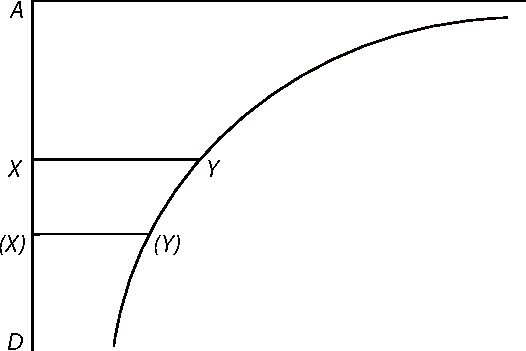
\includegraphics[width=0.55\textwidth]{gesamttex/edit_VIII,3/images/LH_37_01_026_d1.pdf}}%\\
  \vspace{0.5em}
  \centerline{\lbrack\textit{Fig.~1}\rbrack}%
 % \vspace*{1.0em}%
  \newpage% REIN VORLÄUFIG !!!
%
%
\pstart%
\noindent%
Si chorda musica\protect\index{Sachverzeichnis}{chorda musica} $AD$ varie dividatur in punctis $X,$ $(X),$
\edtext{etc.}{%
\lemma{etc.}\Bfootnote{\textit{erg.~L}}}
sonos\protect\index{Sachverzeichnis}{sonus} edet proportionales rectis $XY,$
\edtext{\lbrack$(X)(Y),$\rbrack}{%
\lemma{$(X)Y$}\Bfootnote{\textit{L~ändert Hrsg.}}}
posito $AXD$ esse Asymptoton Hyperbolae $Y(Y),$\protect\index{Sachverzeichnis}{hyperbola}
et $AX$ abscissas, et $XY$ ordinatas.
\edtext{Nam chordae aequabiles aequaliter tensae,\protect\index{Sachverzeichnis}{chorda tensa}
habent}{%
\lemma{Nam}\Bfootnote{%
\textit{(1)}~chorda aequabilis aequaliter tensa, habet
\textit{(2)}~chordae aequabiles aequaliter tensae, habent%
~\textit{L}}}
%
sonos longitudinibus\protect\index{Sachverzeichnis}{longitudo chordae} reciproce proportionales.
Hinc dicimus reciprocos arithmeticorum\protect\index{Sachverzeichnis}{progressio arithmetica}
esse progressionis harmonicae,\protect\index{Sachverzeichnis}{progressio harmonica}
ubi ea est proprietas,
ut \edtext{differentiae trium sint ut extrema.}{%
\lemma{differentiae}\Bfootnote{%
\textit{(1)}~sint
\textit{(2)}~trium sint ut
\textit{(a)}~extrema$\langle$\textsuperscript{rum}$\rangle$.
\textit{(b)}~extrema.%
~\textit{L}}}
\pend%
%
%
\vspace*{2.0em}%
\pstart%
\noindent%
\lbrack\textit{Auf Bl.~26~r\textsuperscript{o}, ohne erkennbaren Zusammenhang mit dem Text:}\rbrack%
\pend%
%
%
%  \newpage% REIN VORLÄUFIG !!!
  \vspace*{2.5em}% REIN VORLÄUFIG !!!
  \centerline{\hspace*{-65mm}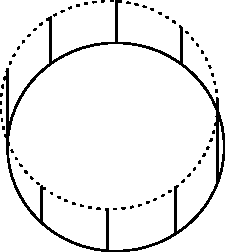
\includegraphics[width=0.20\textwidth]{gesamttex/edit_VIII,3/images/LH_37_01_026_d2a.pdf}}%\\
  \vspace*{0.5em}
  \centerline{\hspace*{-65mm}\lbrack\textit{Fig.~2a}\rbrack}%
\vspace*{-10.0em}%
  \centerline{\hspace*{65mm}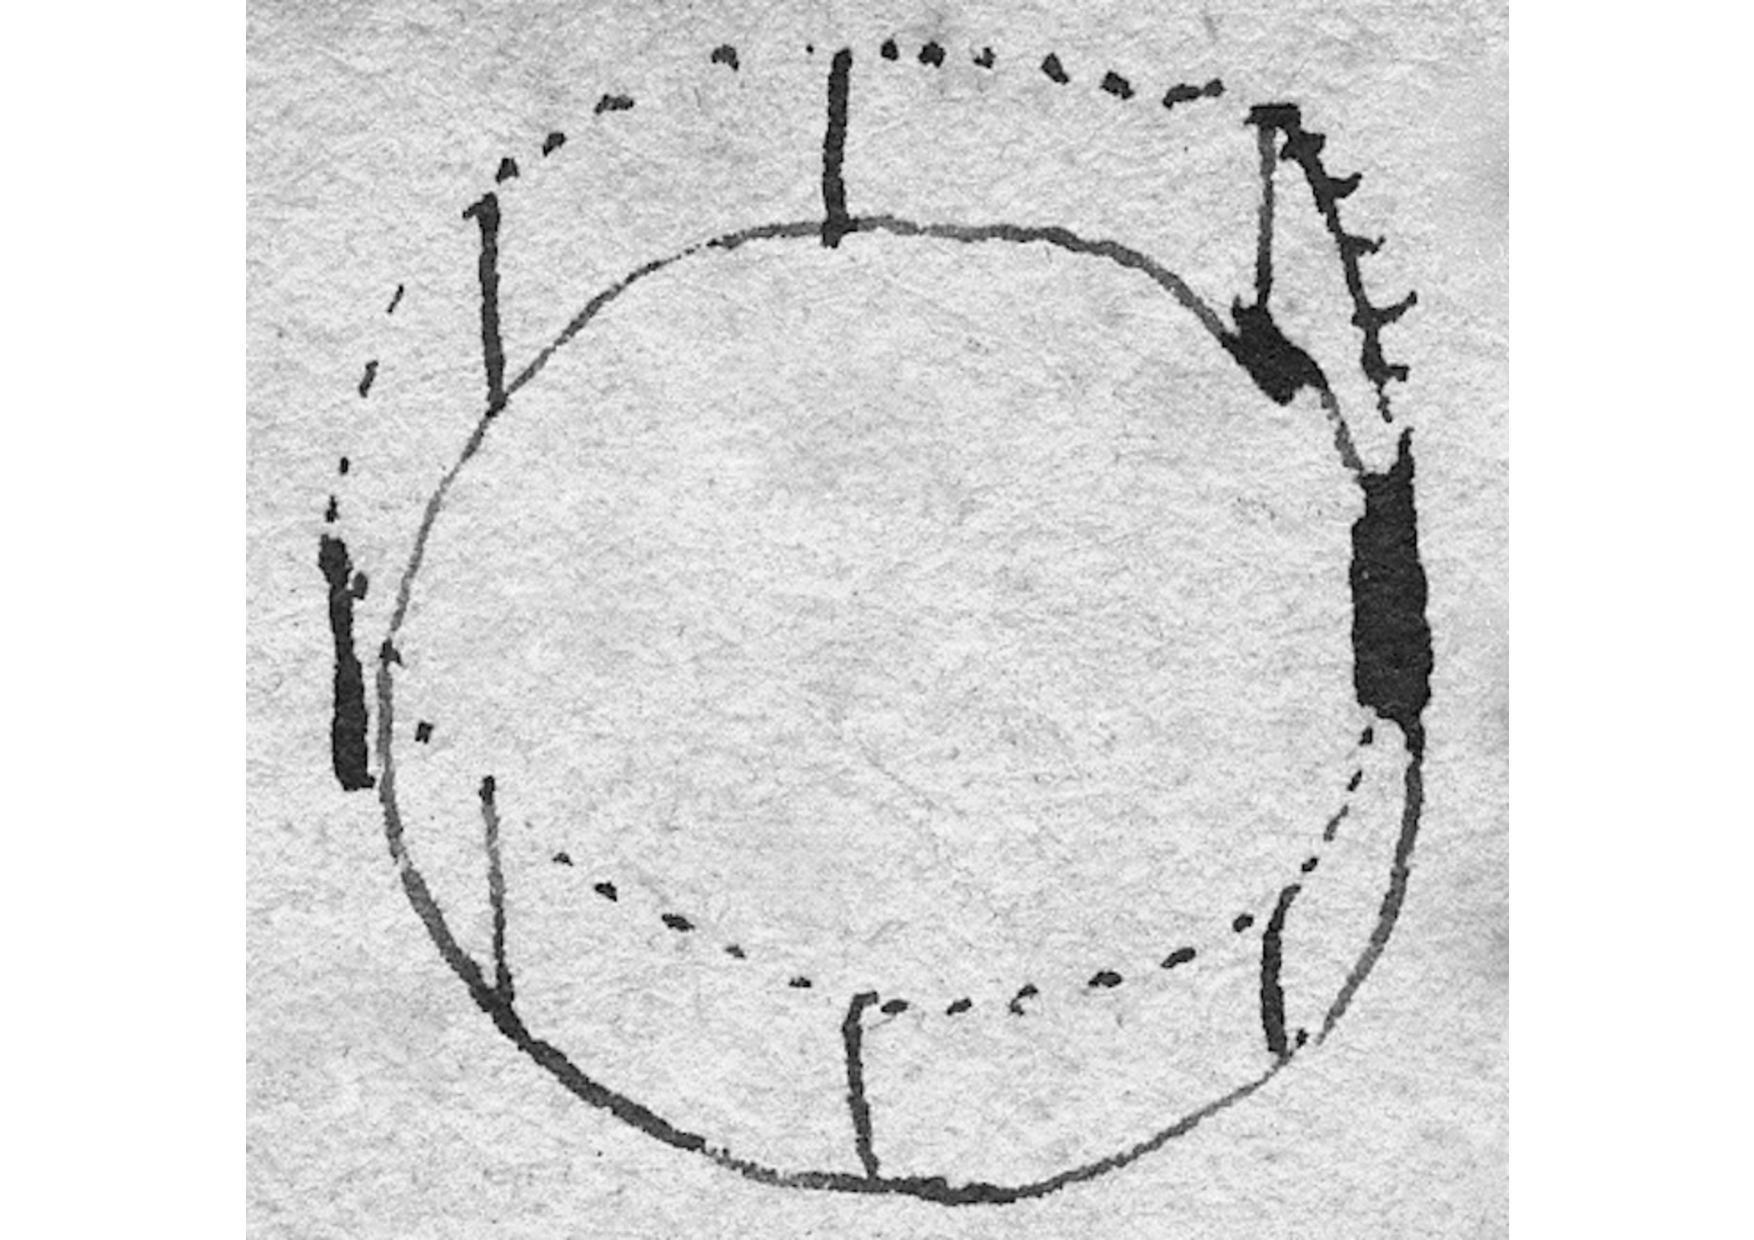
\includegraphics[width=0.30\textwidth]{gesamttex/edit_VIII,3/images/LH_37_01_026_d2b.pdf}}%\\
  \vspace*{0.5em}
  \centerline{\hspace*{65mm}\lbrack\textit{Fig.~2b}\rbrack}%
%  \vspace*{1.0em}%
%  \newpage%
%
%
%%
%  ENDE DES STÜCKES auf Bl. 26r
%%